\label{opti_geom}

\subsection{Prédiction de propriétés moléculaires}

\par Afin de pouvoir prédire les propriétés d'une molécule, les chimistes ont besoin de connaître avec une grande précision la position de son nuage électronique, défini par des orbitales moléculaires. La connaissance de cette information pour les différents niveaux d'énergie d'une molécule permet notamment de prédire les propriétés d'absorption et d'émission de lumière. 
L'étude de l'absorption des molécules est un axe de recherche fort, permettant de prédire leur potentiel photovoltaïque.\\

\par Les orbitales moléculaires sont les solutions d'équations en chimie quantique dont la résolution analytique est impossible. Les chimistes en effectuent donc des approximations à l'aide de fonctions d'ondes, qui sont définies comme la combinaison linéaire de fonctions gaussiennes. Leur calcul est par conséquent un enjeu fondamental en chimie, et est malheureusement très coûteux en termes de puissance et de temps de calcul. Le calcul de la fonction d'onde d'une molécule de taille moyenne d'une cinquantaine d'atomes peut en effet prendre plusieurs semaines.\\

\par La figure \ref{orbitales} représente les iso-valeurs de la fonction d'onde d'une molécule. Les lobes sont proportionnels à la probabilité de présence des électrons.

\begin{figure}
	\centering
	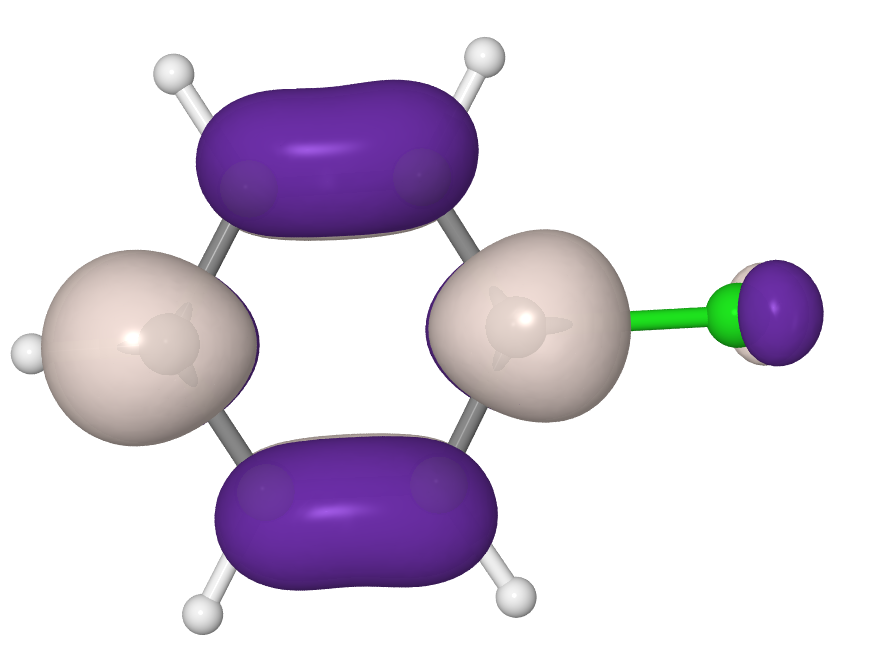
\includegraphics[scale=0.25]{images/iso_niveaux.png}
	\caption{Représentation des surfaces d'iso-valeurs de la fonction d'onde du chlorobenzene\\ (Projet QuChemPedia)}
	\label{orbitales}
\end{figure}


\subsection{Optimisation de la géométrie moléculaire}


\par Les fonctions d'ondes dépendent de la géométrie moléculaire. Les mesures expérimentales géométriques seules ne permettent toutefois pas de les déduire avec suffisamment de précision. Cela est dû au fait que les mesures expérimentales sont effectuées sur un état particulier de la matière. Une phase d'optimisation géométrique par calcul théorique est donc nécessaire.

\par L'approche communément utilisée en chimie quantique pour optimiser la géométrie moléculaire s'appuie sur l'optimisation itérative de la fonction électronique. Il s'agit d'une descente itérative du gradient énergétique des molécules, pour trouver un ensemble de positions atomiques tel que l'énergie totale est minimale, et donc tel que la molécule est la plus stable. Cette méthode est implémentée dans de nombreux programmes de chimie informatique, dont notamment Gaussian, NWChem et Gamess.\\

\par L'inconvénient principal de cette approche est le temps de calcul nécessaire, qui est exponentiellement proportionnel au nombre d'électrons et qui limite donc la possibilité de l'appliquer à des molécules de grandes tailles. Le développement d'une méthode alternative plus rapide et possédant le même niveau de précision ouvrirait donc des perspectives très intéressantes. Il pourrait par exemple permettre la découverte de nouveaux couples de molécules photovoltaïques.
\par Dans l'objectif de réduire le temps d'optimisation, nous souhaitons développer une solution basée sur l'élaboration de modèles d'apprentissage automatique, qui remplaceraient partiellement ou en totalité l'optimisation géométrique quantique.
